
In this chapter, the results and other constraints encountered will be discussed.

\section{Project Management}

Early in the planning and management phase of this thesis, it became evident that the Norwegian infrastructure for retrieving data from various public sources by API was not sufficient for the needs of this thesis. Therefore the initial plan to automate the collection of data needed was adapted to the means of acquiring the data by manually asking the various agencies and implementing their data hard-coded.
\\
This makes the program much less scalable and flexible than hoped for, and severely inhibits future contributions as it may be difficult to couple new data with the inputs of the backend's data structure. The missing automation part will probably hinder future use of this program. The only two APIs used are of American origin, namely Google static map and Twitter. In these regards the automation element that this thesis anticipated failed, however not by a critical means as manual retrieval of data was still possible.






\section{Project resolutions}
In the middle of the time scope for this thesis, a frontend to the backend was desired and thus planning to construct this began. There were several options for choosing not only from the languages the GUI would be based upon but consideration of how a map would be projected as well. These were the main concerns and had to be compatible with each other.
\\
The first choice was between Python's Tkinter GUI module and Node/Javascript GUI. The main reason Python was chosen was that it offered the easiest integration with the backend. Javascript prohibits direct reading from local files, and thus the backend would have to be mounted on a server in order to provide its functions to a frontend. The author of this thesis had little experience with this, and learning a whole new trade was daunting and seemed insurmountable within the rest of the time scope of this thesis, therefore the enticing of the familiarity of Python triumphed. In hindsight, it would probably be better to undertake a Node/Javascript approach because some sort of database to store the backend's data is needed anyway and is probably a more feasible solution. Tkinter is also a framework in which a programmer relinquishes some control for its benefits, this is a minor but notable challenge if it is not familiar.
\\
Choosing a map implementation was difficult, Python has several options like GeoPandas, ipyleaflet, Google static map, cartopy, OpenStreetMap, and basemap. All of the mentioned was hard to install and was sorely limited in function and potential, except OpenStreetMap and Google static map. Upon further investigation Goompy, as described in chapter 2, was discovered and offered a nearly effortless implementation of the map in the already applied design of the frontend.
\\
The advantage the Python solution has is that it requires few installations of external modules and is easily downloaded and mountable on many platforms.
The disadvantage with Python's module Matplotlib, which is used to draw graphs, is that drawing many graphs requires a lot of memory and processor resources, therefore it is important to manage the graphs drawn, and only load those that need be loaded at a time, flushing those that are no longer in use.
The advantage of Google static map is that it is a well implemented and established service with consistent qualitative measures. Google offers fewer road details than OpenStreetMap, and that serves this thesis perfectly as the visualization needed was simply showing locations of traffic registration stations and not necessarily other roads. 
\\
The disadvantages with Google static map is that there are standard usage limits (which can simply be overcome with paying for more). Pixel resolution is set to a maximum of 640x640 pixels, and the free usage is limited to 25.000 map loads per 24 hours. These two limits are not really a problem: The pixel limit is overcome by simply requesting more map loads and then combining those to create as big a picture as desired, and the map loads limit is very high. On average Goompy does 4 map loads per zoom (thus creating a big map of 1280x1280 pixels) and 25.000 / 4 = 6250 zooms per 24 hours, average Norwegian working hours per day is 7.5 hours, this means that one would reach the limit if there are 6.250 / 7.5 / 60 = 13.9 zooms per second. 
\\
This limit was never reached in testing and although it is a high limit if reached the map simply stops working for the remainder of the time to the next 24 hours. Perhaps the most severe limit Google static map have for the scope of this thesis is its maximum URL size of 8192 characters. Figure \ref{fig:google_url} show the programs URL that it sends to the Google map servers, containing a standard map and fifty-three traffic registration stations each with their individually different sizes and colors this surmounts to a total of 4.975 characters already, which is 60.7\% of the total allowed. 

\begin{figure}[!htb]
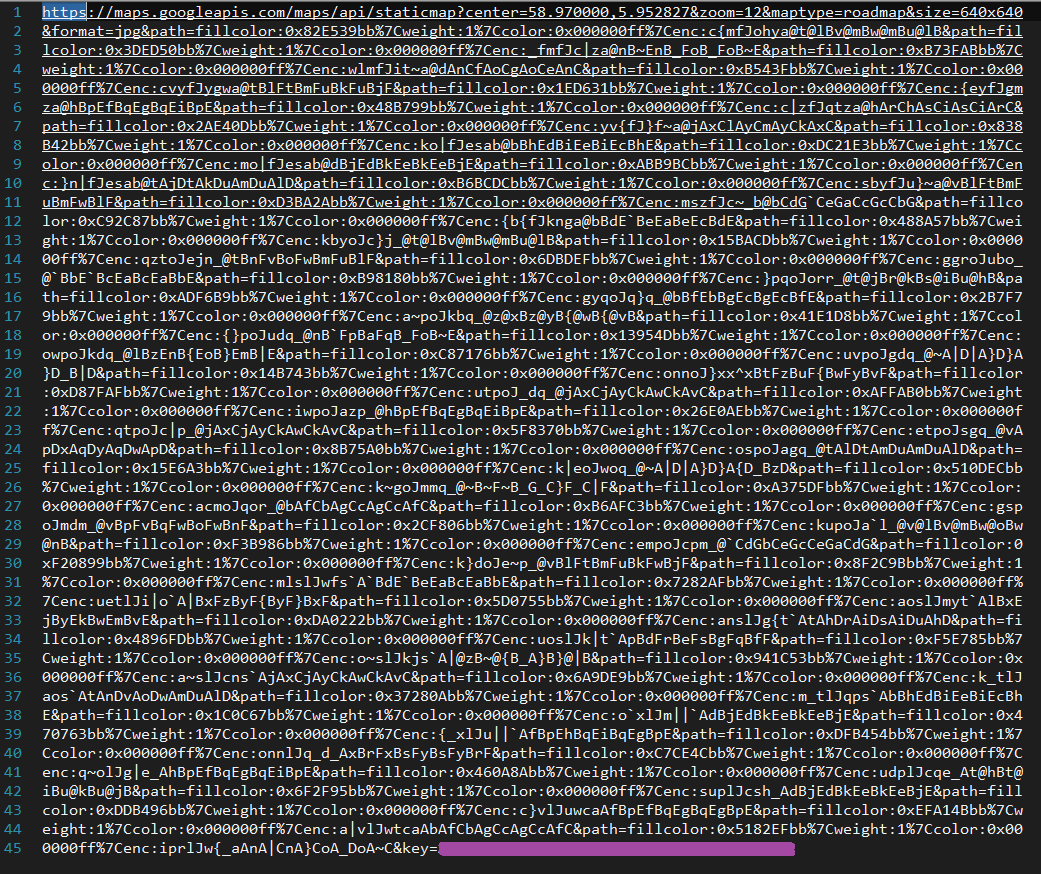
\includegraphics[width=11cm]{Google_static_map_URL}
\centering
\caption{Size of the programs Google static map URL per request.}
\label{fig:google_url}
\end{figure}

Although the url have encoded polylines, which compresses the data, it is already quite long, Loading all of Norway's current 10.066 traffic registration stations using Google static map with this thesis's current algorithms is not feasible, although this could be solved by clustering the traffic registration stations together, and only loading what you actually can see on the map. This would require more Goompy modifications by somehow fetching only those traffic registration stations that are actually currently visible on the map.
\\
The program would still be considered modular and scalable with the chosen technologies and implemented algorithms, although better solutions may be applied.






\section{Ethics}
This potential technology presented is merely a utility information tool that could be used or misused. The question examined is is it acceptable to surveillance the population? And to what extent?
\\
An example of exploit would be the Chinese Sesame 'Social credit system' program\\ \cite{meissner2017china}\cite{china_botsman}\cite{china_wiki}, where a propaganda game rating citizens with 'Sesame credits' on their lives and judging them according to their 'trustworthiness' and 'social integrity' of their individual behaviour. Behaviour such as local and online purchases, real-time location, who friends and family are and what they do, the content of leisure and payment of bills. This mass surveillance tool uses big data analysis technology, and in contradiction to official intents acts as an oppressive system punishing its subjects. Examples of punishment are flight bans limiting movement, excluding parent's children from enrolling in private schools, slow internet access, exclusion from certain jobs, exclusion from hotel services, and forced registration on a public blacklist. The Sesame credit system also works for businesses in their own way.

This thesis does not endorse or suggest oppressive mass surveillance or want to have a consequence of altering peoples behaviour. Unlike the mentioned Chinese system the data used is aggregated, exempli gratia the NPRA data only shows the number of vehicles passed and in no way can trace individual behaviour. A system for detecting influenza does not need data on an individual level, but the Chinese system depends on individual data and analysis with intent to influence a person's etiquette.


It is considerate to contemplate ethical values when developing systems that rely on public information extraction, taking care to not be reckless with sensitive data by insincere or cynical means, and having a genuine interest in the well-being of the public without consequences of oppression or discrimination. This is the reason the NIPH ILI daily data from Oslo and Bergen are omitted in the delivery of this thesis even though the data is aggregated beyond identification, as the possible information derived might be too delicate, and also possibly protected by Norwegian confidentiality laws. Norway already has a government agency installed protecting such concerns\cite{datatilsynet}, albeit new technologies and usage are revealed continuously it is important to have an ongoing update on such policies.













\section{Future works}
The program contains bugs and inefficient solutions, ameliorating these algorithms requires more work than what is this thesis's time scope. There is a multitude of different open sources, tools, and frameworks in existence. Choosing the right technology and solution for the right project and problem is a challenging task that perhaps becomes easier with experience and adequate knowledge. The willingness, endurance, and eagerness to learn a new contrivance ultimately persuade productivity, though missteps are a menace. The state of ever-changing available technologies makes it so viable options change rapidly, and the adherence to adapt is an ever-evolving developer skill. This thesis could have been better served with additional forethought which would require supplemental research on applied standardisation and feasible solutions to structure and wanted features. Although the presented work is within the desired outcome, better realisation of necessities and accessibilities may have been further advantageous.

\subsection{Known bugs and other imperfect implementations}
One known negligent solution is the algorithms in the program of double\_y\_graphs.py where redundant calculations take place. Fixing this would make the program gui.py slightly faster and be more structural preferable. The difficulty lies with not reusing already created objects and instead forge a new, this is in probity a crude imposition underneath expected proficiency.\\
The program NIPH\_frame.py serves the function to present two graphs on the same x-axis and with their own separate y-axes, this was however only accomplished on a weekly temporal resolution. Some graphs have a higher resolution like for instance Twitter, but the data is still aggregated into a weekly resolution in the program. Writing algorithms that would support an hourly or weekly resolution became outside of the time scope of this thesis. Future work may focus on being able to compare different resolutions as this would offer a better comparison of the different datasets.\\
Another known bug is that the buttons panel disappear when the window size is not big enough, the attempt to amend this has again and again produced frustration and the answer remains to this day a mystery.
The NPRA hourly dataset GUI implementation is missing the option to choose from different traffic registration stations. One reason this was not prioritised in time was that the data obtained was in an older data structure and conversion was difficult, though the one available hourly data set in the program proves the concept of manipulating and studying the NPRA statistics.\\
Some functions in the different modules both in the backend and in the frontend are redundant, a better overall structure would be to collect these often used functions in their own utility module. An example of this may be the drawing of graphs in the backend. Having a draw module that only draws whatever the different modules require would serve as a uniform utility tool. This was implemented lastly in the frontend with the program constants.py which only serves the shared constants for the color theme. This makes it easy to change because one would only have to alter it in one place, not having the need to search through every place it is implemented in code. A solid utility module for both the backend and the frontend should have been achieved for better structure and optimisation.

\subsection{Google static map}
As discussed in the previous chapter clustering traffic registration stations would solve the maximum URL problem. When presented with a map that shows all of Norway instead of showing each traffic registration stations one could cluster them together by proximity, and when zooming in present an even more fine-tuned clustering until the zoom level is sufficient enough to show all of the traffic registration stations on that level. This is already a standard way of presenting spatial data as seen in the NPRA's online roadmap\cite{vegkart} when selecting multiple elements. Further standardising colors and sizes would significantly save url length, the thought behind different sizes and colors was only intended on a very zoomed in level and is not necessarily needed when showing clusters. Considering when and what is needed amends the complication. The url size problem would also completely vanish if taken a Node/Javascript approach instead. 

\subsection{Database}
At the very end of the time scope of this thesis, it became obvious that the backend's data should have been implemented in some sort of a database in order to speed up the process of reading and extracting exact information, this especially relevant for the NPRA hourly dataset. Data filtering is the process of refining data sets for relevant user information, different filters can be tailored to different needs. Filtering becomes particularly useful in the NPRA's hourly dataset, an example would be to filter out the different vehicle lanes available, this would on average make the algorithm two times faster. In order to take advantage of data filtering and indexing the data would have to be implemented in a database. A possible more optimal solution would be to rewrite the entire project to Node/Javascript and mount the backend's data on a server such that it is available to the frontend modules.

\subsection{Test driven development}
Test-driven development (TDD) is the exercise of writing tests for code even before the creation of the algorithm to be tested upon. The goal is to specify the exact parameters and functions an algorithm should have by writing a test firstly, and then writing the actual algorithm and making it pass the test. Although this is a big investment that essentially adds another layer of complexity and requires continuous tweaking the advantages are imposing. A clear acceptance criteria safely define the purpose should one be left astray, and convey a focus on integration, control and well-organized code for safer refactorisation and fewer bugs. The toll of utilizing TDD is high inherently but quickly offers increasing returns and is a virtuous investment that also serves as a living document.
In hindsight, it is the belief that this thesis would benefit greatly from this practice, and should be considered a future contrivance if this thesis should ever be rewritten by others.

\subsection{Additional features}
A wanted feature was the variance calculation of the different traffic registration stations that had hourly dataset on them. This would visualize the data on the map in an interestingly manner by differing the sizes based on amount of traffic and colourise them based on the difference by each station's yearly variance. This planned feature fell of of this thesis's time-scope, and although outlined never reach actualisation. There are however attempted experimental algorithms in the program NPRA\_Traffic\_Stations\_load\_data.py, the main concern was the time-cost of these algorithms as calculating the variance of one hourly dataset over the course of five years meant reading through about 87.630 lines of data which could take nearly a minute to run on modern computers. This is why having an indexed database would be beneficial when running such an algorithm on all of the 53 traffic registration stations accessible in this thesis. Although a neat feature the lack of a indexed database and insufficient time, this was never completed.


